\documentclass[a4paper,10pt,twocolumn]{article}

\usepackage{graphicx}
\begin{document}
\title{\emph{blkin}: An end-to-end tracing tool for software defined storage 
systems}
\date{}
\maketitle

\section*{Abstract}
Distributed storage systems require special treatment concerning their 
monitoring and tracing because of their low-latency and high-throughput demands.
In this paper we describe the development of a low-impact, live tracing 
infrastructure used in monitoring of large scale storage systems. \emph{blkin}
is a system based on LTTng\cite{lttng} implementing the tracing scheme proposed
in the Dapper paper\cite{dapper}. Our contribution to the problem includes a 
tracing library based on the Dapper semantics targeting low-latency applications
as well as a proposed architecture for live tracing of such kind applications.
As a usecase of our system, we decouple and analyze Archipelago\cite{archip} and
RADOS\cite{rados} measure read/write requests initiated with the VMs that end up
being served by RADOS.


\textbf{Keywords: } tracing, monitoring, low-latency, LTTng, RADOS

\section{Introduction}

The recent burst of cloud computing has made distrubuted systems much more 
popular. However, debugging or monitoring a distributed system is a difficult 
and demanding job. Dealing with multiple hosts makes the system's behavior 
unpredicatable and bound to a specific context. Thus, finding failures
or bottlenecks cannot be achieved through traditional performance analysis or 
debugging tools. 

This problem can be tackled through tracing. Tracing captures the state of the
system along with other needed information that could provide further insight of
the exact context that a specific event happened. These information can be 
correlated so as to explore the system's behavior under different working 
states. In order to obtain, this kind of information, various instrumentation
points should be placed in the system's source code informing about the state
that an event happened.

Tracing a distributed system can be very challenging and various 
problems may arise. The system should be traced under real working conditions,
since most of the failures are about to appear then. So, the tracing mechanism
should not affect significantly the system's performance. Also, since we want to
explore a distributed system's behavior, we have to deal with multiple hosts and
events happening almost simulataneously. This sets two different challenges.
How to qualitatively correlate event information and how to quantitatively 
correlate time information between different hosts. For the first problem, all
the traces concerning a specific initial request should be gathered togather
no matter where they were logged. For the second problem, since we approach 
performance analysis as well, the tracing mechanism should take into
consideration the time differences between the hosts' clocks. These differences
may be crucial when analyzing time latencies.

Some of the most widespread distributed systems are the distributed storage
systems. These systems can be used either as huge data warehouses for images,
videos etc, or as storage backends for virtual volume provisioning for IAAS 
providers. In any case, their performance analysis and tuning is of vital
importance since large latencies may end up to an unresponsive system and user
disatisfaction. In order to debug and monitor such storage systems we need to 
tackle the aformentioned problems.

In this paper, we present the design and implementation of \emph{blkin}.
\emph{blkin} is a system that enables us to debug and monitor through tracing
a distributed storage system in real time, with a very low overhead and 
visualize the aggregated information. This information, caming from cross-layer 
tracing, enables us to explore the system's behavior under various circumstances
and workloads, since we have at our disposal an accurate, end-to-end
representation of the request's route from the time it enters the system till
it is finally served. This enables us to explore the time latencies between the
different layers and the possible bottlenecks that our system may have. In order
to fulfil the previous prereqisites, we make use of \emph{LTTng} (Linux Trace 
Toolkit - next generation)\cite{lttng} for low overhead tracing and the tracing
schema used in Google's Dapper for tracing information correlation.

As a usecase, we are using \emph{blkin} in tracing a software defined storage 
system \emph{Archipelago}\cite{archip}. Archipelago is used by Synnefo 
\cite{synnefo}, an IAAS provider software and uses RADOS\cite{rados} as storage
backend. Concequently, with \emph{blkin} we trace the IO requests from the time
they are created within the VM, till they are finally served by RADOS.

\section{Tracing logic}
One of the most important aspects of system tracing is the aggregated 
information correlation and interpretation. There are two dominant schools 
concerning tracing information. \emph{Black box} monitoring scheme assumes there
is no additional information other than the message record. So statistical 
regression techniques should be used to infer any existent association. 
\emph{Annotation-based} schemes, on the other hand, rely on applications or 
middleware to explicitly tag every record with a global identifier that links 
these message records back to the originating request. In order to have an 
overall review of the system per specific request, we have to implement an 
annotation-based monitoring scheme.

After examining the nature of distributed storage systems, we found some common
characteristics that should be taken into consideration when designing an
end-to-end tracing infrastructure.
\begin{itemize}
\item Every request in order to be completed passes through \textbf{different 
phases} in order to get served. Each phase implements a different functionality.
Between these distinct phases there is communication overhead crucial to the 
system's performance that needs to be measured. 
\item Throughout the serving of the request, \textbf{different nodes} of the 
infrastructure are activated. These nodes may vary depending on the request.
Information about the exact time and place of a trace record should also be 
kept.
\end{itemize}

Google proposed a complete annotation-based monitoring scheme in the Dapper 
paper\cite{dapper}. This proposed scheme enables us to depict casual
relationships between the different processing phases. In short, Dapper 
describes the following semantics for tracing:
\begin{description}
\item[annotation]
The actual information being logged. There are two kinds of annotations. Either
\emph{timestamp}, where the specific timestamp of an event is being logged or 
\emph{key-value}, where a specific key-value pair is being logged.
\item[span]
The basic unit of the process tree. Each specific phase of processing can be 
depicted as a different span. Each span should have a specific name and a 
distinct span id.
\item[trace]
Every span is associated with a specific trace. A different trace id is used 
to group data so that all spans associated with a specific trace also share the
common trace id. For our case, information concerning a specific request to the
storage system share the same trace id and each distinct request initiates a new
trace id.
\item[parent span] 
In order to depict the causal relationships between different spans in a single
trace, parent span id is used. Spans without a parent span ids are  known as 
\emph{root spans}.
\end{description}

So, by creating tracing data according to these semantics we can have an 
end-to-end sense of our system's performance, behavior and internal latencies
that may vary depending on the nature and size of each request.

\subsection{Logic implementation}
Based on these primitives, Twitter created Zipkin\cite{zipkin}, a distributed
tracing system used to gather timing data for all the disparate services 
running on their premices. Zipkin consists of a data collector, a database 
service and a Web interface to vizualize the aggregated data created according 
to the principles described above.

Zipkin uses Scribe\cite{scribe} to transport all the traces from the different
services. Scribe is a logging server created by Facebook, aiming to be scalable
and reliable. Scribe servers are arranged in a directed graph, with each server
knowing only about the next server in the graph. This network topology allows
for adding extra layers of fan-in as a system grows, and batching messages
before sending them between datacenters as well as providing reliability in case
of intermittent connectivity or node failure. Scribe makes use of 
Thrift\cite{thift} for data transfer

Zipkin seemed to fit our demands concerning data collection since it is designed
to scale. Also, the used SQL-schema was adequate to capture and query all the 
needed tracing information and finally, the Web UI offered us descriptive 
visualization of the traces, apart from the SQL-interface used for more 
elaborate queries. Although Zipkin offers various libraries (Python, Ruby, 
Scala) in order to instrument applications, there was no providence for 
low-latency applications written in C/C++. Our contribution was to create a 
C/C++ library that encapsulates the Dapper semantics and can be used within 
C/C++ projects to create trace information in accordance with the aformentioned
logic. This library is designed to be backend-independent, which means that one
can implement his own log aggregation backend for the library. However, we 
offered a specific backend implementation according to our initial prerequisites 
concenring overhead that is being thoroughly examined in the next chapter.

\section{Low overhead tracing}
As mentioned before, a storage system's performance is a crucial matter. Both 
throughput and latency should be uneffected by tracing. So every approach to 
monitor or trace this kind of systems should have the least possible added 
overhead to the instrumented application which should continue working properly
production-wise. Traditional logging systems would fail to tackle this problem,
since they tended to separate the tracing from the operational phase.

\subsection{Tracing backend}
\emph{blkin} was designed driven by a strict low-overhead prerequisite. So the 
first important decision to make concerned the system that would implement the
system's backend, namely the system that would run on every cluster node and 
would be responsible for aggregating tracing data from the instrumented 
applications. So we chose to use \emph{LTTng} (Linux Trace Toolkit - 
next generation)\cite{lttng} in our system backend.

\emph{LTTng} is a toolchain that allows integrated kernel and user-space tracing
from a single user interface. \emph{LTTng} was initially designed and 
implemented to reproduce, under tracing, problems occurring in normal 
conditions. It encapsulates synchronization primitives that meet the low-impact
requirements by using a linearly scalable and wait-free RCU (Read-Copy Update) 
synchronization mechanism. This mechanism was also ported from the kernel to 
userspace. In addition, \emph{LTTng} supports a variety of operating systems
(Debian, Fedora, Arch) and since version 2.x kernel tracer modules are built 
against a vanilla or distribution kernel, without need for additional patches.
So, \emph{LTTng} enabled us to use the same generic toolkit for both user and 
kernel tracing and it could be easily installed on almost every system needed
to instrument. 

However, unlike other similar tracing systems (eg. SystemTap\cite{systemtap})
that follow a different approach and are not suitable for monitoring, LTTng adds
the least possible overhead to the tracing system. LTTng supports static 
tracepoint instrumentation. This means to manually insert tracepoints in the 
application source code and rebuild the application. After rebuilt, these 
tracepoints will breakpoint-less and system-call-less produce the described 
traces as far as userspace is concerned. As far a kernel-space is concerned, 
LTTng is supported by kprobes and kernel markers. Thus LTTng does not 
significantly affect the system's performance and is ideal to for the C/C++
tracing library mentioned before.
Although the whole process of recompiling the instrumented application  may seem
counterproductive, static instrumentation abilities are limitless. Based on the
knowledge and understanding of the application, one can instrument and trace 
every part that might be problematic or causing longer latencies, as well as 
extracting all the information needed to fully understand the system's context.
Consequently, static tracing match our tracing needs, since we want to trace in
accordance with the Dapper semantics.

\subsection{Live tracing}
In order to locate possible problems and analyze the performance of a large 
distributed system, tracing should happen while the system is in production.
All the vulnerabilities, faults, or bottlenecks would become obvious under this
kind of tracing. This would mean to trace a production system and in real time 
have access and process the aggregated information, without separating the 
tracing from the operating phase. Although this may sound natural for 
traditional logging systems like syslog, in combination with the demand for
low-impact tracing, several difficulties arise. Older approaches required 
separation between the tracing and operation phases. This happened either 
because tracing added a lot extra overhead to the instrumented system, or 
because tracing information was not in a state that could be processed before 
the end of the tracing session. For LTTng especially, tracing data were in a 
binary form and could be decoded only after the end of the tracing session. 

\subsubsection{Infrastructure}
Since version 2.4 of \emph{LTTng}, live tracing is possible. Tracing 
data can be streamed, decoded and processed processed in real time in different
using a daemon process called \emph{relayd} that collects the tracing data over 
the network using batch TCP packets.  

However, \emph{LTTng} live tracing supports only its native CTF format. 
Consequently, in order to be able to process and visualize tracing data in real
time with Zipkin, we needed to implement a live-tracing plugin that would 
transform real time CTF data to Scribe messages sent to either a local or the
central Zipkin Scribe server. So based on Babeltrace\cite{bltrace}, which is a 
CTF converter and trace viewer, we developed a plugin that reads and decodes the
CTF-formatted information, it creates Thrift\cite{thrift} encoded messages 
recognizable by the Zipkin collector and sends these messages to the Scribe 
server. So we end up with the architecture presented in figure 1.

The instrumented application produces tracing information according to the 
Dapper semanctics using our custom made tracing library, through instrumentation
points in its source code. These information are aggregated by \emph{LTTng} and
sent to the \emph{relayd} daemon. This daemon runs either on the same or on a 
different node. After that, our Babeltrace plugin communicates with the 
\emph{relayd}, gets the tracing data, processes them as mentioned and finally 
sends the data to the Scribe server. 

\subsubsection{Deployment}
In figure 1 each arrow represents a TCP communication. This offers us a lot of 
versatility concerning deployment. Based on specific needs and cluster 
architecture each service can run on a different node.  Also, the Scriber server
that the Babeltrace plugin finally sends the tracing information can be either 
the central Zipkin collector or a local Scribe daemon that will eventually send
the data to the central collector, thus exploiting the 
asynchronous, buffered communication provided by Scribe.

So in a cluster deployment with many nodes, we end up having the architecture
presented in figure 2. In this deployment, there is a whole \emph{blkin} stack 
running on every node of the cluster. All the communication is over localhost 
and there is also a local Scribe daemon. This daemon will store data locally in
case of a connection loss with the central server or if the central zipkin 
collector is busy. So we can make sure that no data will be lost, because any
data loss would mess up the tracing semantics and end up with an inconsistent UI
and database state.

%\begin{figure}[h!]
%  \centering
%  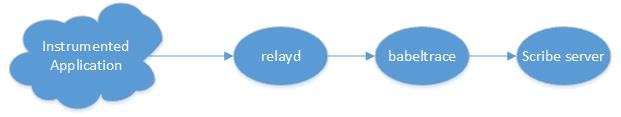
\includegraphics[scale=0.75]{images/specific.jpg}
%  \caption{\emph{blkin} architecture}
%\end{figure}
%
%\begin{figure}[h!]
%  \centering
%  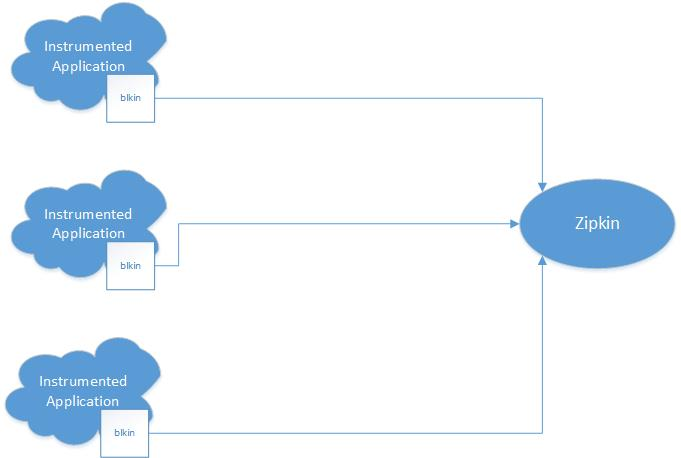
\includegraphics[scale=0.75]{images/generic.jpg}
%  \caption{\emph{blkin} deployment}
%\end{figure}

\section{Time Synchronization}

A crucial matter that needs special treatment when it comes to distrubuted 
tracing is time synchronization. In a \emph{blkin} cluster deployment, ideally
we would like to have no time difference between the cluster nodes' clocks, 
since we are interested in measure latencies and processing durations in the 
scale of nanoseconds. So, a possible time skew in the scale of microseconds 
could result in having a request response virtually happening before its request.

In order to solve this problem various solutions have be proposed in the past.
Before June 2010, when NTP version 4 was published, NTP's precesion was within
the interval from 100 $\mu$s to 2 ms. Such precision was unacceptable for
tracing storage systems. So statistical methods were developed. Time skews were
approximated using arichmetic analysis methods like linear regression. In these
methods, each node collected traces using its own clock and afterwards, after
calculating the time differences from a specific node considered anchor, these
deltas were applied to the traced time information. According to \cite{hp} these
methods performed well. However, the disadvantage of these methods was the post
processing overhead which could be significant for long tracing sessions and the
fact that live tracing was not possible.

However, the new version of NTP (verion 4) published in June 2010 improved NTP's
synchronizing potential accuracy to the tens of microseconds with modern 
workstations and fast LANs. According to our measures,....
So, using one cluster node as a NTP server, thus exploiting the fast LAN 
interconnecting the cluster nodes, we can achieve the needed time accuracy.
 
\section{Evaluation - Usecase}

In order to evaluate our system and our tracing model's expressiveness, we 
instrumented \emph{Archipelago}\cite{archip}. Archipelago is a distributed 
storage layer that decouples Volume and File operations/logic from the actual
underlying storage technology, used to store data and is part of the Synnefo 
project\cite{synnefo}. Although Archipelago supports several storage backends,
we chose to use and instrument RADOS\cite{rados}. 

Through this instrumentation we expect to identify and measure the different 
logic layers through which a user read or write request passes from the time of
its creation till the answer reaches back to the user, as well as the enclosed 
latencies between them.

\begin{thebibliography}{9}
\bibitem{rados}
    RADOS: A Scalable, Reliable Storage Service for Petabyte-scale
    Storage Clusters
\bibitem{archip}
    Archipelago,
    info about
\bibitem{lttng}
    LTTng,
    info about
\bibitem{systemtap}
    SystemTap,
    info about
\bibitem{bltrace}
    Babeltracep,
    info about
\bibitem{dapper}
    Dapper,
    info about
\bibitem{zipkin}
    Zipkin,
   info about
\bibitem{scribe}
    scribe,
   info about
\bibitem{thrift}
    scribe,
   info about
\bibitem{synnefo}
    scribe,
   info about
\bibitem{hp}
    hp paper
\end{thebibliography}
\end{document}
